\documentclass[12pt,fleqn,leqno,letterpaper]{article}
\usepackage{graphicx}
\usepackage{hyperref}
\graphicspath{{../figures/}}

\title{Luminosity}
\author{Cameron, M. \and Rosales, V. \and Westermann, J.P.}

\date{July 30, 2017}

\begin{document}

\maketitle
\newpage
\tableofcontents
\listoffigures
\listoftables

\newpage

Notes (Please Read):
\begin{itemize}
  \item print(df.to\_latex()) will give a latex export of the dataframe in the jupyter notebook, you can use this to quickly copy paste into latex
  \item plt.savefig(<path>) will allow you to save your figure as a png so it can be used in the document/presentation
  \item Make sure to commit and pull as much as possible to avoid merge errors
  \item Don't edit the styles of this document yet, will do that at the end
\end{itemize}

\begin{section}{Introduction}
  \begin{subsection}{Summary}
    TODO Will do this last
  \end{subsection}
  \begin{subsection}{Literature Review}
    \begin{subsubsection}{Luminosity-based Approach}
      TODO Michael: Try to accumulate as much as possible. We have such a long list of papers anyway.
    \end{subsubsection}
    \begin{subsubsection}{Natural Disaster Economics}
      TODO Viviana: obviously, as the expert.
    \end{subsubsection}
  \end{subsection}
\end{section}

\begin{section}{Data}
  \begin{subsection}{Data Description}
    TODO Micheal: Describe what the data looks like, how many observations there are, where we got it, who else has used it etc.
  \end{subsection}
  \begin{subsection}{Data Preprocessing}
    \begin{description}
      \item[Volume]{While the number of observations is extremely low, as only annual images are available from 1992 to 2013, the dimensionality of each observation (image) is considerable. With a size of $16801$ by $43201$, every image contains $725820001$ pixels in total, which results in more than 700MB of disk-space required for only one image in uncompressed format. This also means that computations on the entire dataset are not possible with common personal computing architecture.}
      \item[Diverse Sources]{To aggregate meaningful information to use in the model, such as economic indicators from the world bank (gdp, import, export, inflation, etc.), we need to join data from a lot of different sources on different aggregation levels.}
    \end{description}
    \begin{subsubsection}{QGIS}
      TODO Viviana
    \end{subsubsection}
    \begin{subsubsection}{Python Architecture}
      To enable exploration and flexible modelling of the data even on a platform where memory and computing power are quite restricted, we built a supporting architecture in python for loading the images and aggregating the features. To quickly load entire time series of the most important places, the sections of the image representing the biggest cities and a 150x150 area around them are cut out and stored as seperate time series. This allows for more easilty training predictive models for the luminosity. Additionally, functions where created to easily load a 'section' time series (the series of images for one particular subsection of the world's image), given coordinates and the desired size of the image. The stored data is no longer in the `tif` format provided at download. All images have already been passed into arrays and stored as compressed numpy arrays. That reduces the required storage space by an order of magnitude. The functions to preprocess and load the data can be found in the \hyperref[www.github.com/westermann/luminosity]{GitHub repository}.
    \end{subsubsection}
    \begin{subsubsection}{Denoising}
    \end{subsubsection}
  \end{subsection}
\end{section}

\begin{section}{Modelling}
  \begin{subsection}{Disaster Impact Models}
    Exploratory analysis and some basic models are a first step to assessing the impact of natural disasters on the luminosity time series. For this, we need to make a modelling decision regarding how the disaster (represented only as a single point location) can be geospatially associated with pixel luminosity values. TODO Jonas, literature on this?
    \begin{subsubsection}{Linear Distance-based Modelling}
      One practical mathematical choice is a function decaying with distance affecting areas or even individual pixels on the grid. The advantage of this method is that it is simple to explain, easily tuneable and leaves a lot of flexibility for modelling. Additionally, it captures the notion that areas in the vicinity of a disaster event are more likely to be affected than those further away by default.
      We trialed this approach using the luminosity data in combination with TODO (NGOAAASDF Name?). We extracted 150x150 squares from the satellite image of the entire planet in a similar fashion as a convolutional neural network would apply to an image. Then we filtered the top $t\%$ most luminous 'subimages', as we can generally disregard those parts of the world that contain no lights (oceans, deserts, etc.) and calculate a disaster coefficient based on a function decaying linearly with distance. The $t$ percentage threshold can be tuned in order to keep the data small enough to process. This is necessary as in practice,  means calculating the distance between every section of the image's center and every earthquake and then applying a linear function of the distance and the magnitude for every earthquake that occurs in a given year, then summing up these effects to generate a disaster impact variable for that observation. This results in a high computational load as for every section that we extract from the image, we need to compute the eucledian distance to every singe one of the 25000 earthquakes, making in almost infeasible on a common laptop. However, already only the luminosity growth between beginning and end of the image time series and the disaster coefficient show promising qualities of the data when plotted agains one another.
      \begin{figure}
        \centering
        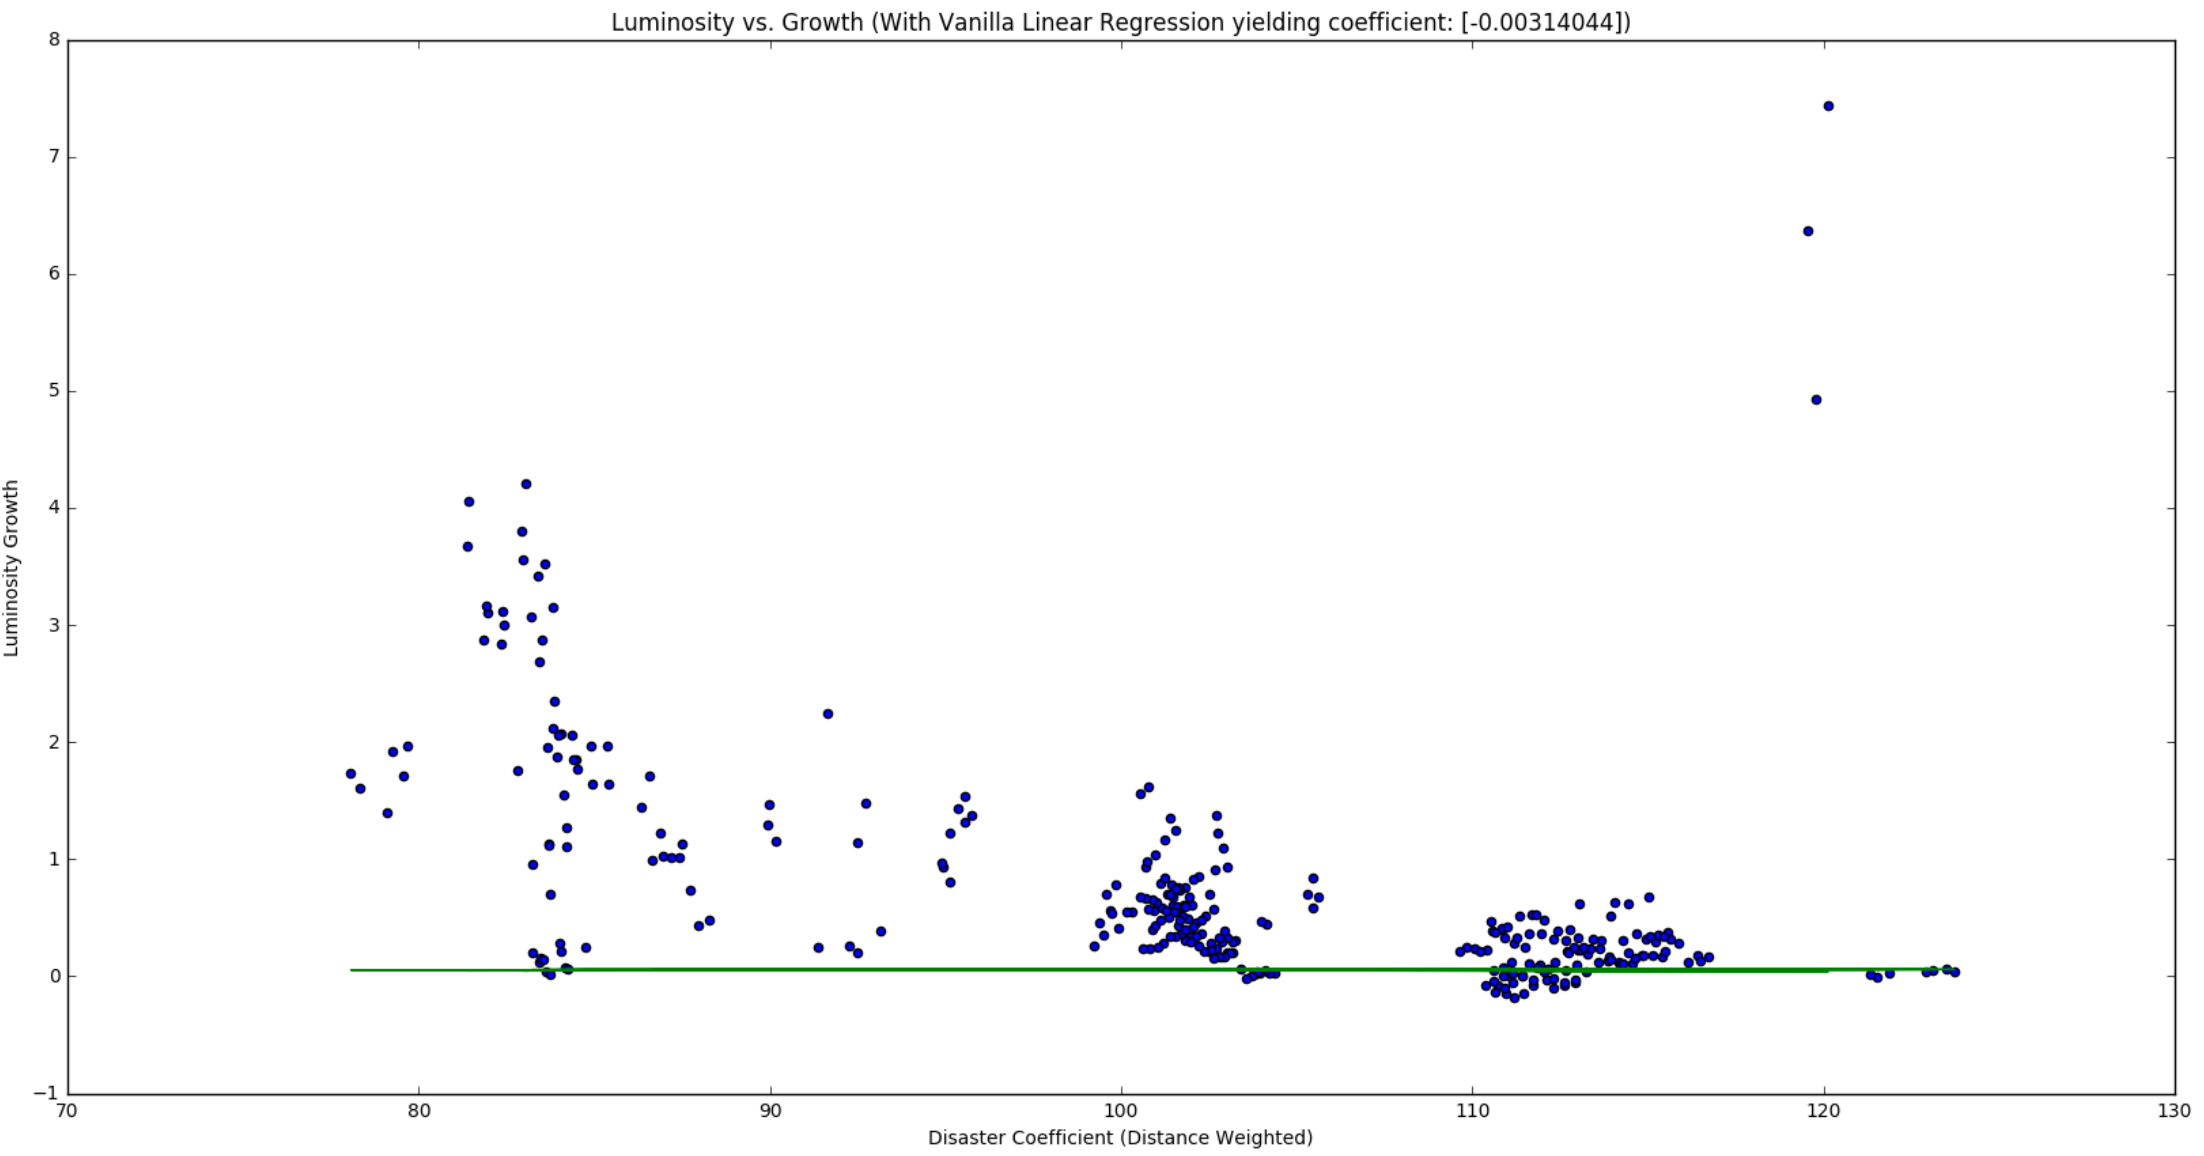
\includegraphics[width=1\linewidth]{linear-model-1}\label{fig:linear-model-disco-vs-lum-growth} %TODO: Adjust plot pngs to have sensible size for document
        \caption{Luminosity Growth 1992-2013 plotted against a linearly decaying disaster coefficient for 150x150 image sections.}
      \end{figure}
      However, this approach makes some strong assumptions about the nature of natural disasters that don't hold in reality. An important factor in how much impact a disaster has on a region are geographical features: An earthquake will affect different areas differently based on their rockbed and geological consistency while e.g.\ storms and floods depend strongly on the topography. Nevertheless, the calculation of such a disaster coefficient yields promising results and suggests there is a relationship in the data between disaster coefficient and the growth in a location, proxied by luminosity.
    \end{subsubsection}
    \begin{subsubsection}{Recorded Disaster Impact-based Modelling}
      Another possible approach, that is commonly applied in Economics, is to use institutional data on which cities where affected by an earthquake. Using the TODO datasets we can obtain records of cities that were affected by a given earthquake in a given year. Matching this with a simple list of the world's largest 50000 cities, we can obtain a panel dataset that associates earthquake damage without any measure of magnitude to cities, some affected, others not.
      We can then 
    \end{subsubsection}
    \begin{figure}[t!]
      \centering
      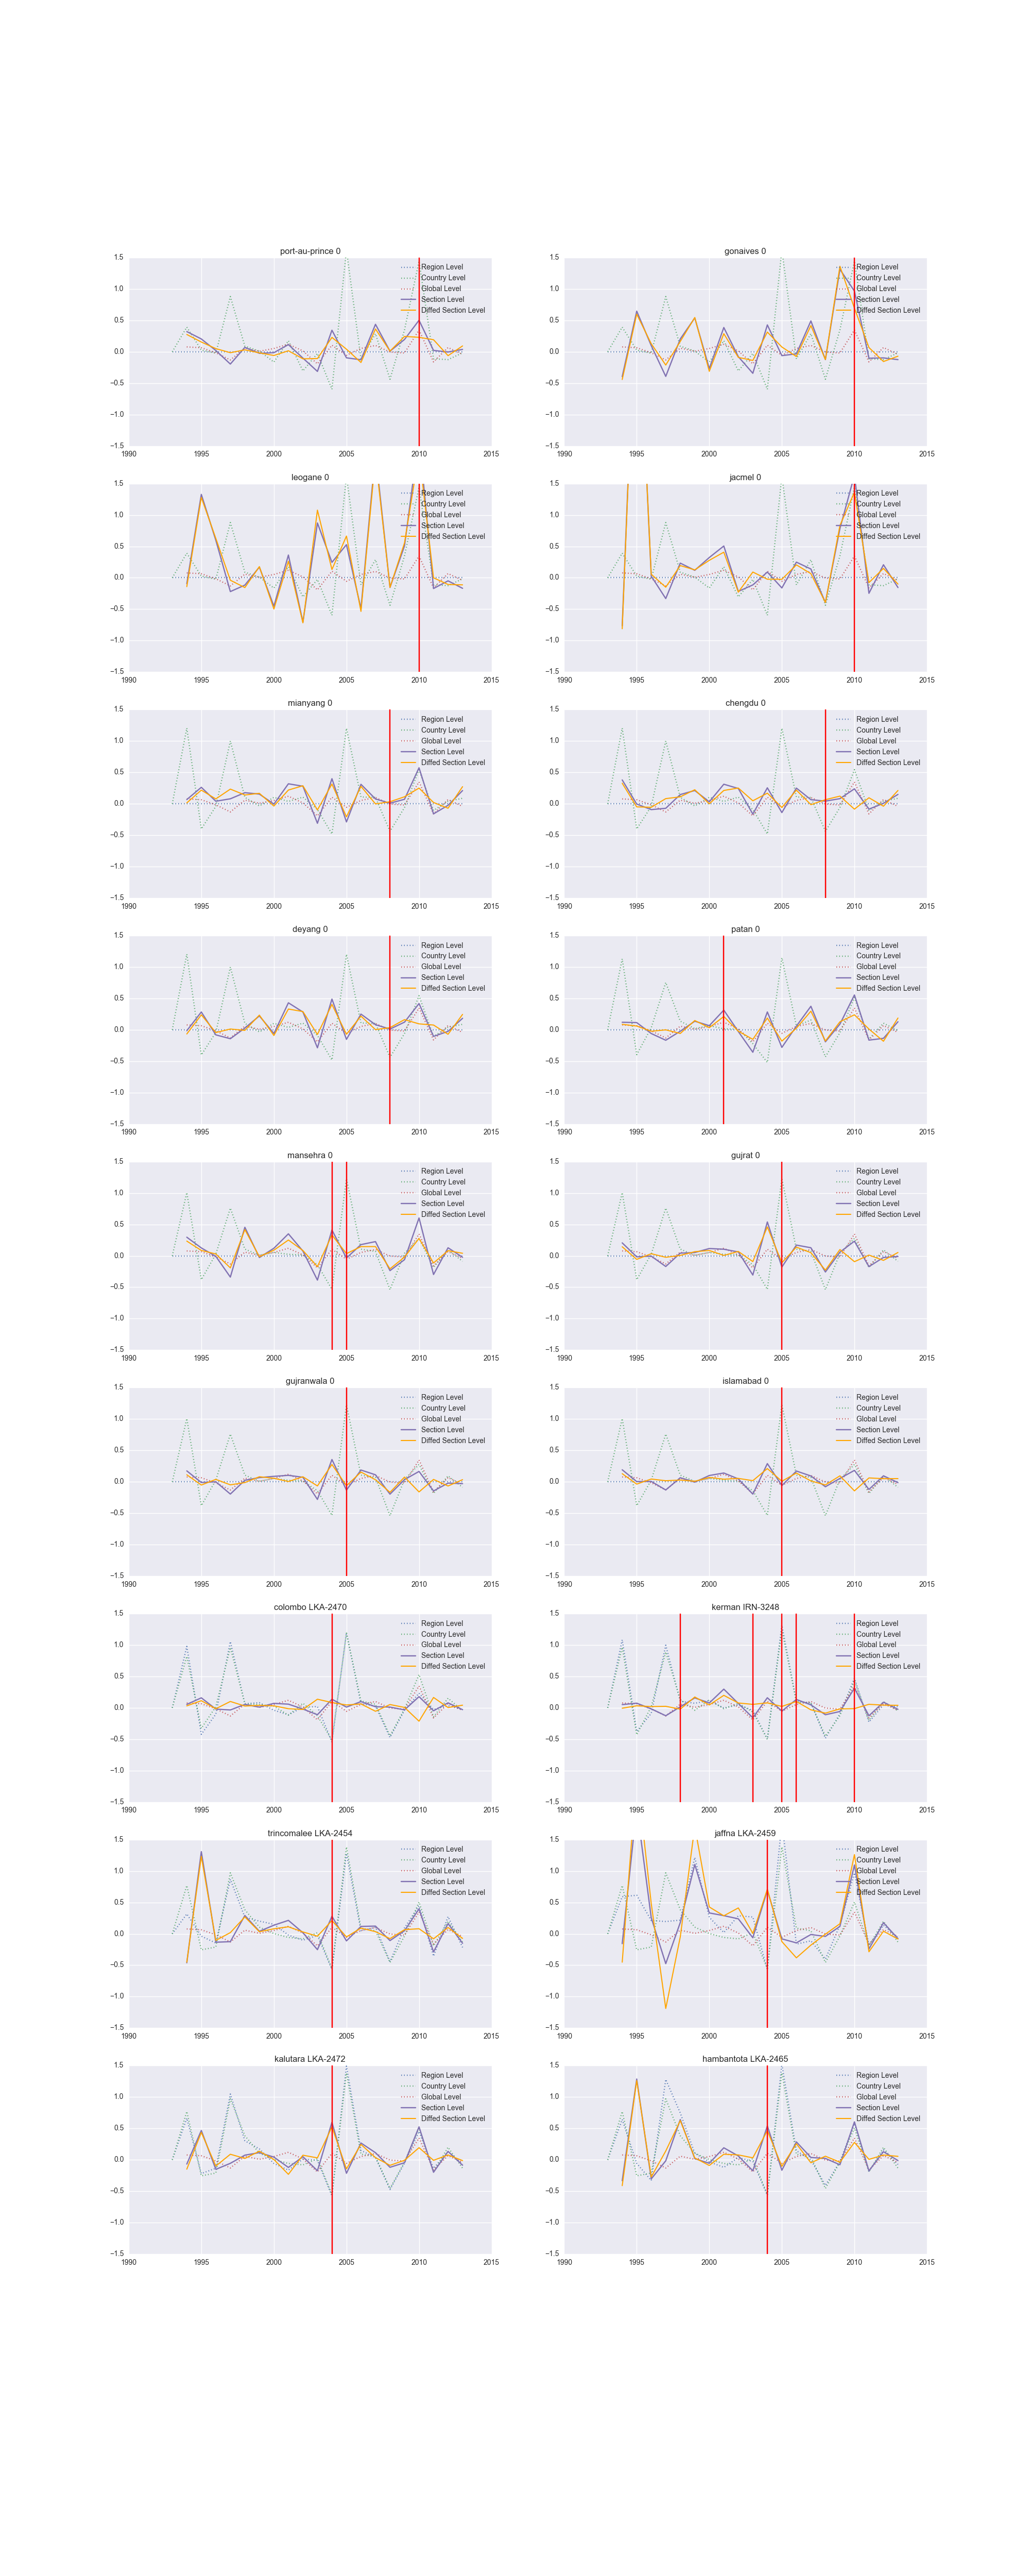
\includegraphics[width=1\linewidth]{pca_balancer_diffs}\label{fig:weighted_balanced_luminosity_sum_series} %TODO: Adjust plot pngs to have sensible size for document
      \caption{Luminosity Series Balanced by PCA Components}
    \end{figure}
    \begin{figure}[t!]
      \centering
      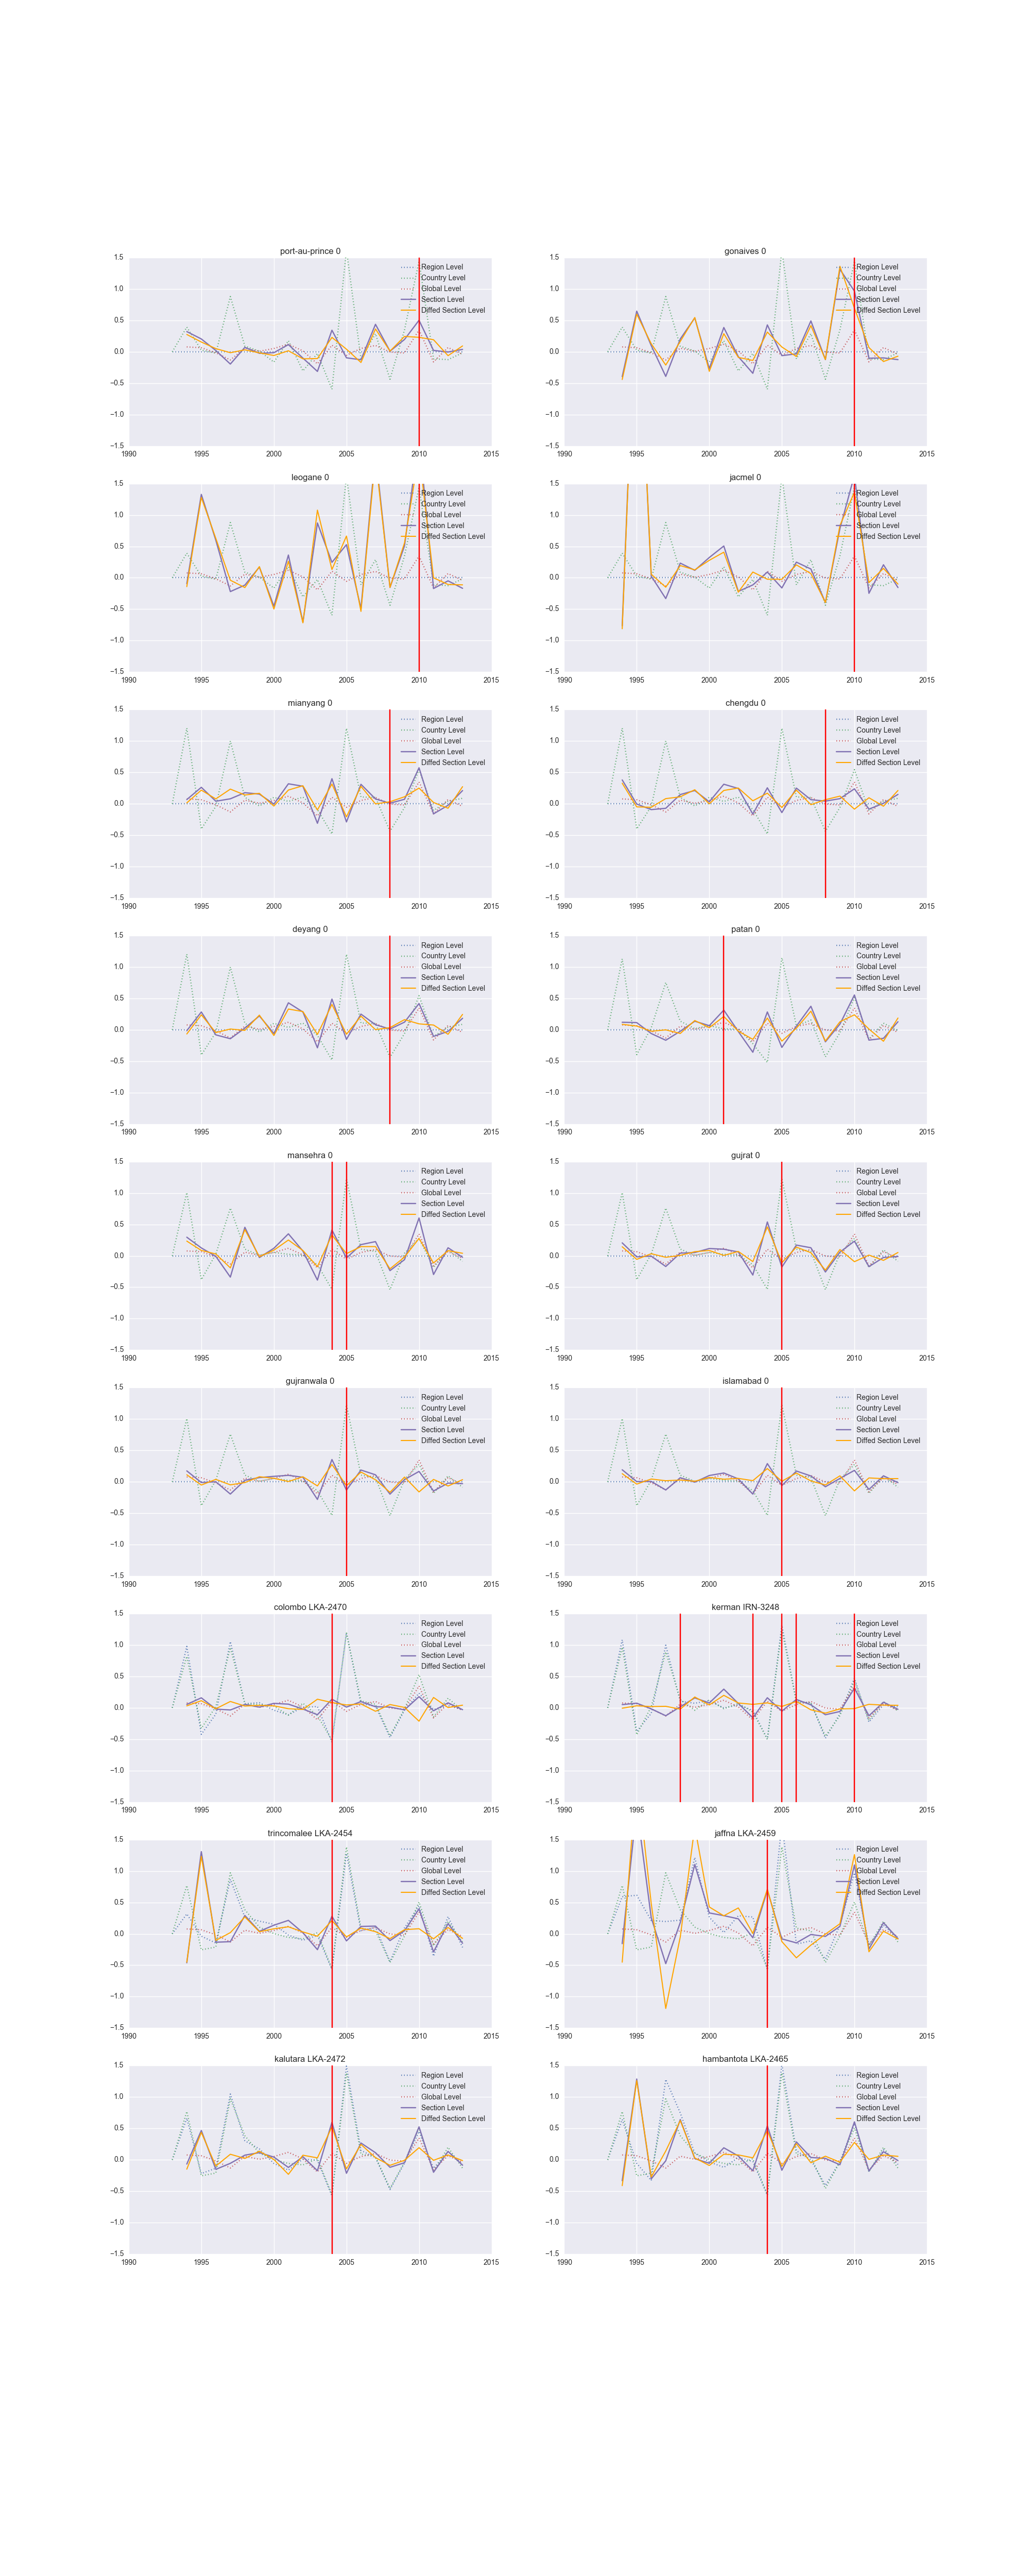
\includegraphics[width=1\linewidth]{pca_balancer_diffs}\label{fig:pca_balanced_luminosity_sum_series} %TODO: Adjust plot pngs to have sensible size for document
      \caption{Luminosity Series Balanced by PCA Components}
    \end{figure}
  \end{subsection}
  \begin{subsection}{Panel Model}
    \begin{subsubsection}{Region-based Panel}
      TODO Viviana
    \end{subsubsection}
    \begin{subsubsection}{Section-based Panel}
      TODO Jonas
    \end{subsubsection}
    \begin{subsubsection}{Dynamic Panel}
      TODO Viviana: Describe here how the model that you are using is constructed, where you got it, etc.
    \end{subsubsection}
  \end{subsection}
\end{section}

\begin{section}{Results}
  \begin{subsection}{Case Analysis}
    TODO Micheal: This is where your case analysis for different places goes, try to add some statistical tests etc.\ if possible. E.g.\ distribution of light one year vs the next compared to overall time series distribution changes (shocks).
  \end{subsection}
  \begin{subsection}{Modelling Results}
    TODO Viviana: Describe the results of the regression here, significant values and what those values mean.
  \end{subsection}
  \begin{subsection}{Conclusions}
    TODO Will do this just before the summary
  \end{subsection}
  \begin{subsection}{Outlook}
    TODO Jonas
  \end{subsection}
\end{section}

% -- Bibliography (APA style)
\bibliography{references}

\end{document}
